\documentclass[14pt, a4paper, ukrainian]{extreport}

\usepackage[14pt]{extsizes}
\usepackage{cmap}
\usepackage[utf8]{inputenc}
\usepackage[T2A]{fontenc}
\usepackage[english, ukrainian]{babel}
\usepackage{slashbox}
\usepackage{caption}
\DeclareCaptionLabelFormat{gostfigure}{Рисунок #2}
\DeclareCaptionLabelFormat{gosttable}{Таблиця #2}
\DeclareCaptionLabelSeparator{gost}{~---~}
\captionsetup{labelsep=gost}
\captionsetup*[figure]{labelformat=gostfigure}
\captionsetup*[table]{labelformat=gosttable}
\captionsetup*[figure]{labelformat=gostfigure, justification=centering}  % выравнивание по центру



\usepackage{titlesec}

\titleformat{\chapter}[block]
{\filcenter}
{\thechapter}
{1em}
{\MakeUppercase}
{}

\titlespacing*{\chapter}{0pt}{-40pt}{*4} 

\titleformat{\section}
{\filright}
{\thesection}
{1ex}{}


\title{Розрахункова робота № 1}
\author{Олександр Вергелюк}
\date{\today}


\usepackage[left=3.00cm, right=1.50cm, top=2.00cm, bottom=2.00cm]{geometry}

%Робота з математикою 
\usepackage{graphicx}
\usepackage{amsmath, amsfonts, amssymb, mathtools} %AMS
\usepackage{icomma} %Розумна кома
\usepackage{indentfirst}
\parindent 1.25cm
\usepackage[usenames,dvipsnames]{color}
\usepackage{makecell}
\usepackage{multirow}
\usepackage{ulem}
\usepackage{float}

%Шрифти
\usepackage{euscript}
\usepackage{mathrsfs}
\linespread{1.3} % полуторный интервал

%Власні команди
\DeclareMathOperator{\sgn}{mathop{sgn}}

%Перенесення знаків у формулах (За Львовським)
\newcommand*{\hm}[1]{#1\nobreak\discretionary{}%
	{\hbox{$\mathsurround=0pt #1$}}{}}

\begin{document}
	\begin{titlepage}
	\centering
	\vspace{1cm}
	{ МІНІСТЕРСТВО ОСВІТИ І НАУКИ УКРАЇНИ\\
		НАВЧАЛЬНО-НАУКОВИЙ КОМПЛЕКС\\
		``ІНСТИТУТ ПРИКЛАДНОГО СИСТЕМНОГО АНАЛІЗУ``\\
		НАЦІОНАЛЬНОГО ТЕХНІЧНОГО УНІВЕРСИТЕТУ УКРАЇНИ\\
		``КИЇВСЬКИЙ ПОЛІТЕХНІЧНИЙ ІНСТИТУТ ІМЕНІ ІГОРЯ СІКОРСЬКОГО``\\
		КАФЕДРА МАТЕМАТИЧНИХ МЕТОДІВ  СИСТЕМНОГО АНАЛІЗУ\\\par}
	\vspace{5cm}
\Large \MakeUppercase {\textsc{\textbf{{розрахункова робота №1}}}}\\
\Large {з теорії ймовірності} \\
на тему: {<<Випадкові вектори>>}\\
Варіант 7
\vfill
\newlength{\ML}
\settowidth{\ML}{\hspace{3.4cm}}
\hfill
\begin{minipage}{0.4\textwidth}
	Виконав студент 2 курсу групи КА-06\\
	Вергелюк Олександр Андрійович
	
	Перевірив: \\
	Ільєнко А. Б.
\end{minipage}
\vfill
\begin{center}
Київ -- 2021
\end{center}
\end{titlepage}
	\chapter{Завдання 1}
	
	Нехай дискретний випадковий вектор $\vec\xi = (\xi_1, \xi_2)$ задано таблицею розподілу (Таблиця {\ref {tab:task1}}).
	
	\begin{table}[H]
		\caption {\label{tab:task1} Таблиця розподілу вектора $\vec \xi$}
		
		\begin{center}
			\resizebox*{!}{!}{
				\begin{tabular}{ | c | c | c | c | c | }
					\hline
					\backslashbox {$\xi_1$}{$\xi_2$} & -9 & 2 & 7 & 8\\
					\hline
					-2 & 0.17 & 0.01 & 0.07 & 0.06 \\
					\hline
					1 & 0.13 & 0.08 & 0.04 & 0.08 \\
					\hline
					2 & 0.12 & 0.02 & 0.07 & 0.15 \\
					\hline
				\end{tabular}
			}
		\end{center}
	\end{table}
	
	\section{Ряди розподілу координат $\xi_1$ та $\xi_2$}
	
	Для $\xi_1$ використаємо формулу: $ p_i = \mathbb{P} \{\xi_1 = x_i\} = \sum_{j = 1}^{n} p_{ij}$.
	
	\begin{table}[H]
		\caption{\label{tab:xi1} Ряд розподілу $\xi_1$}
		\begin{center}
			\resizebox*{!}{!}{
				\begin{tabular}{| c | c | c | c |}
					\hline
					$x_i$ & -2 & 1 & 2 \\
					\hline
					$p_i$ & 0.31 & 0.33 & 0.36 \\
					\hline
				\end{tabular}
		}
		\end{center}
	\end{table}
	
	Перевірка: 	$$ 0.31 + 0.33 + 0.36 = 1$$	
	Аналогічно для $\xi_2$: $ p_j = \mathbb{P} \{\xi_2 = y_j\} = \sum_{i = 1}^{m} p_{ij} $.
	
	\begin{table}[H]
		\caption{\label{tab:xi2} Ряд розподілу $\xi_2$}
		\begin{center}
			\resizebox*{!}{!}{
			\begin{tabular}{| c | c | c | c | c |}
				\hline
				$y_i$ & -9 & 2 & 7 & 8\\
				\hline
				$p_i$ & 0.42 & 0.11 & 0.18 & 0.29\\
				\hline
			\end{tabular}
		}
		\end{center}
	\end{table}

	Перевірка:  $$ 0.42 + 0.11 + 0.18 + 0.29 = 1 $$

	\section{Функції розподілу $F_{\xi_1}(x)$ і $F_{\xi_2}(y)$ та їх графіки}
	
	Для координати $\xi_1$:
	
	$$ F_{\xi_1} =  \begin{cases}
		0  & x \le -2\\
		0.31 & -2 < x \le 1\\
		0.64 & 1 < x \le 2\\
		1 & 2 < x
	\end{cases}
	$$
	
	\begin{figure}[H]
		\centering
		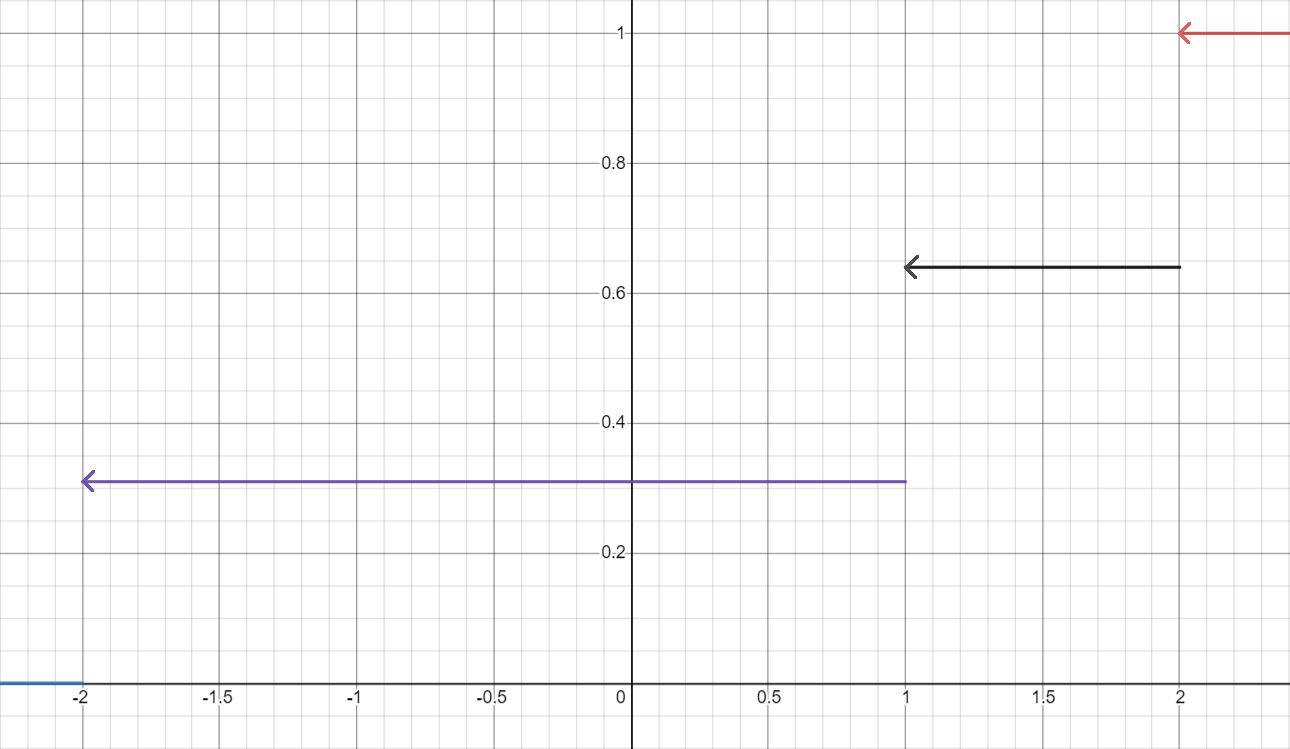
\includegraphics[width=\textwidth]{./Image/Im_01_Fx.png}
		\caption{Функція розподілу $F_{\xi_1}(x)$}
		\label{im:Fx}
	\end{figure}

	Для координати $\xi_2$:
	
	$$F_{\xi_2}(y) = \begin{cases}
		0 & y \le -9\\
		0.42 & -9 < y \le 2\\
		0.53 & 2 < y \le 7\\
		0.71 & 7 < y \le 8\\
		1 & 8 < y
	\end{cases}
	$$

	\begin{figure}[H]
		\centering
		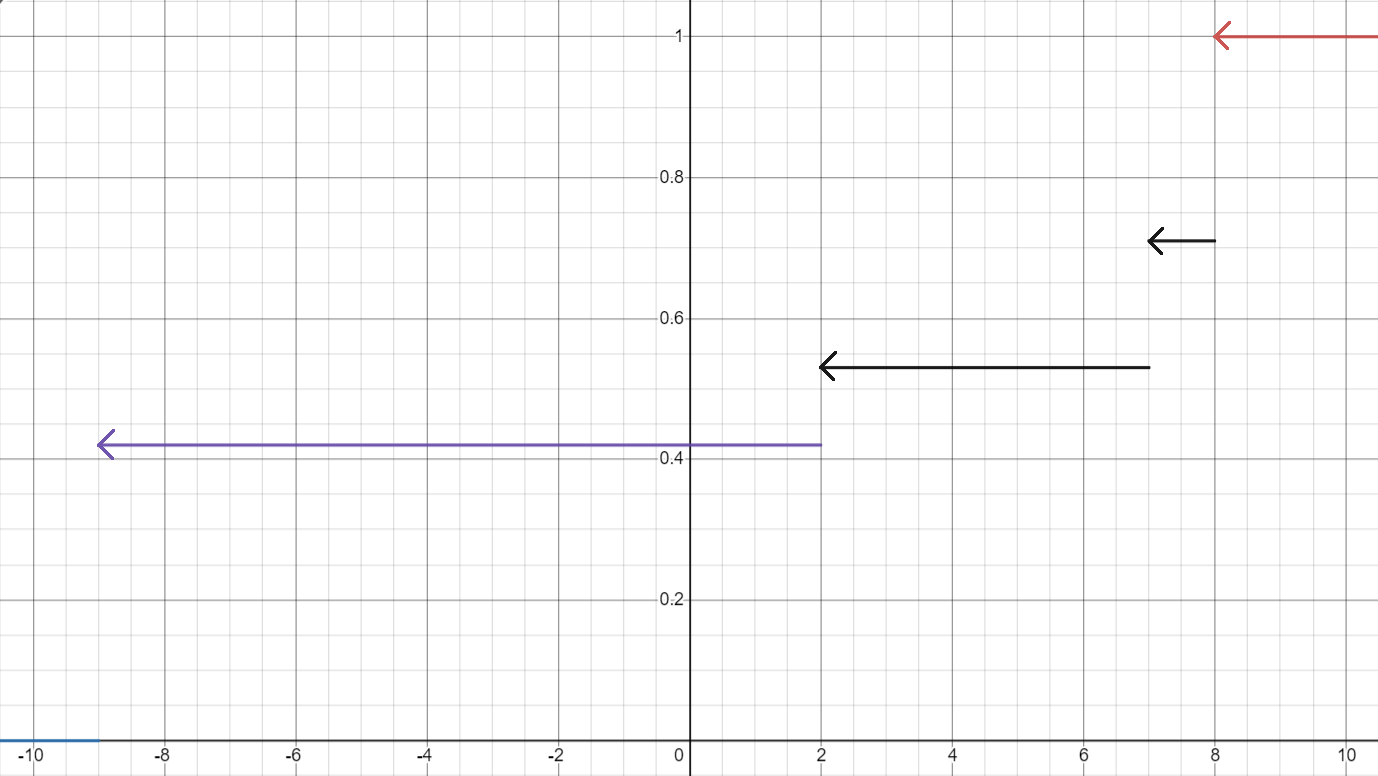
\includegraphics[width=\textwidth]{./Image/Im_02_Fy.png}
		\caption{Функція розподілу $F_{\xi_2}(y)$}
		\label{im:Fy}
	\end{figure}
	
	
	\section{Функція розподілу $F_{\vec \xi}(x, y)$ випадкового вектора}
	
	Зобразимо в декартовій системі координат всі точки, що відповідають значенню вектора $\vec \xi$ (рис. \ref{im:Fxy}).

	\begin{figure}[h!]
		\centering
		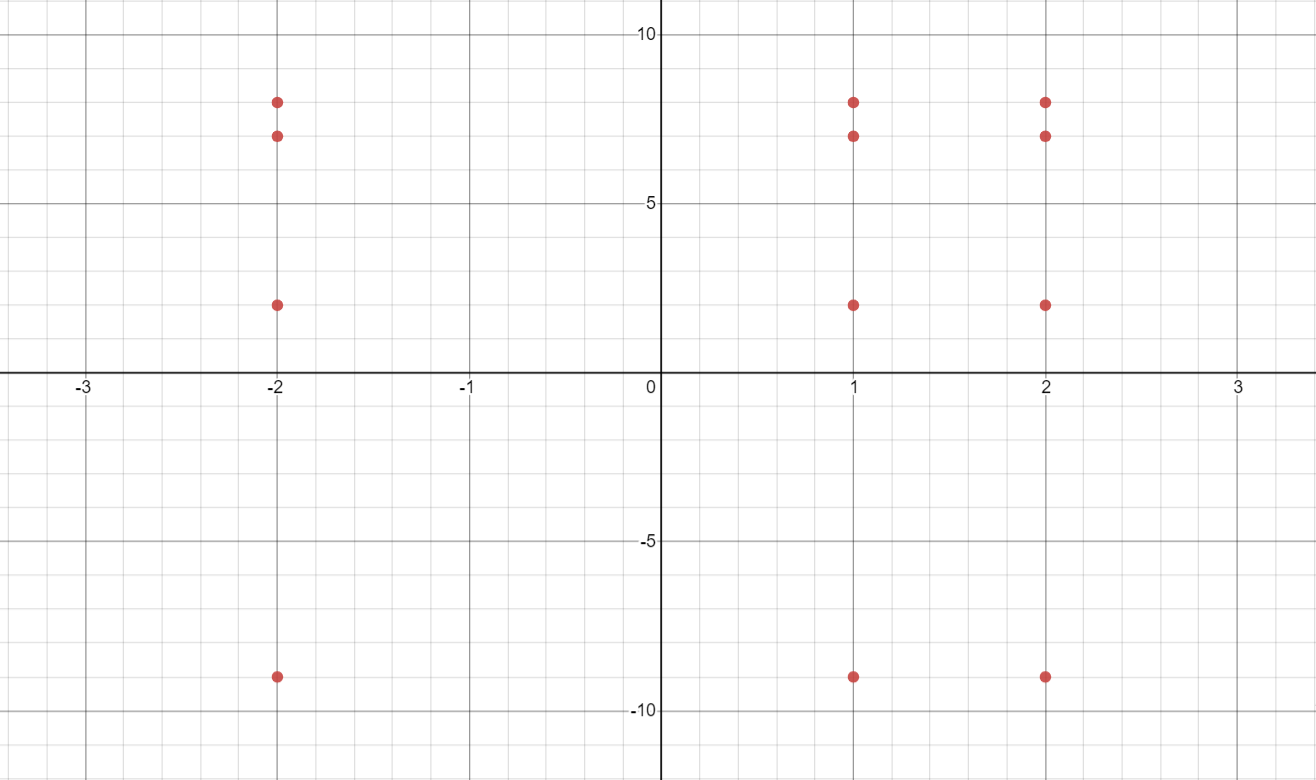
\includegraphics[width=\textwidth]{./Image/Im_03_Fxy_1}
		\caption{Значення вектора $\vec \xi$ в декартовій системі координат}
		\label{im:Fxy}
	\end{figure}

	Розіб'ємо координатну площину на області, в яких сумісна функція розподілу $F_{\vec \xi}(x, y)$ набуває однакові значення (рис. \ref{im:Fxy_D}).
		
	\begin{figure}[h!]
		\centering
		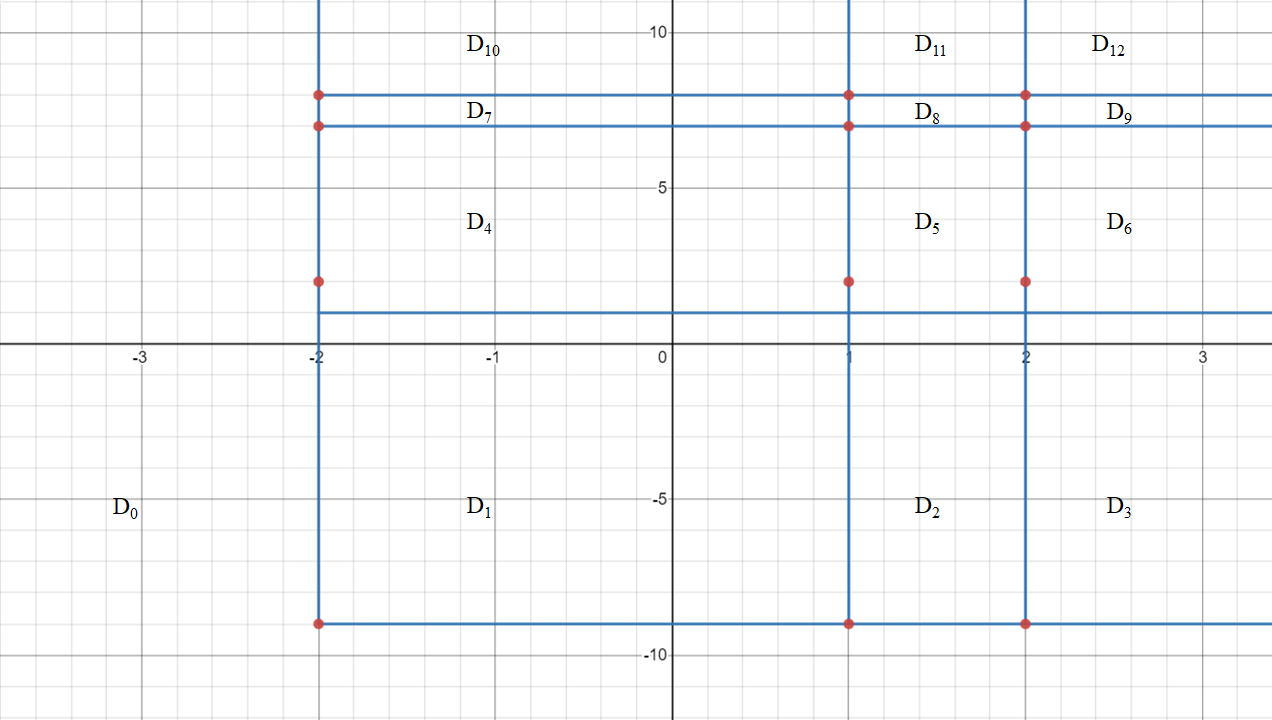
\includegraphics[width=\textwidth]{./Image/Im_04_Fxy_2}
		\caption{Області, в яких сумісна функція розподілу $F_{\vec \xi}(x, y)$ набуває однакові значення}
		\label{im:Fxy_D}
	\end{figure}

	Використаємо формулу:
	$$ F_{\vec \xi }(x, y) = \mathbb{P} \{\xi_1 < x, \xi_2 < y\} = \sum_{i:x_i < x} \sum_{j:y_j = y} p_{ij}$$
	a) $(x, y) \in D_0 \Rightarrow F_{\vec \xi}(x, y) = 0$\\
	b) $(x, y) \in D_1 \Rightarrow F_{\vec \xi}(x, y) = 0.17$\\
	c) $(x, y) \in D_2 \Rightarrow F_{\vec \xi}(x, y) = 0.3$\\
	d) $(x, y) \in D_3 \Rightarrow F_{\vec \xi}(x, y) = 0.42$\\
	e) $(x, y) \in D_4 \Rightarrow F_{\vec \xi}(x, y) = 0.18$\\
	f) $(x, y) \in D_5 \Rightarrow F_{\vec \xi}(x, y) = 0.39$\\
	g) $(x, y) \in D_6 \Rightarrow F_{\vec \xi}(x, y) = 0.53$\\
	h) $(x, y) \in D_7 \Rightarrow F_{\vec \xi}(x, y) = 0.25$\\
	i) $(x, y) \in D_8 \Rightarrow F_{\vec \xi}(x, y) = 0.5$\\
	j) $(x, y) \in D_9 \Rightarrow F_{\vec \xi}(x, y) = 0.71$\\
	k) $(x, y) \in D_10 \Rightarrow F_{\vec \xi}(x, y) = 0.31$\\
	l) $(x, y) \in D_11 \Rightarrow F_{\vec \xi}(x, y) = 0.64$\\
	m) $(x, y) \in D_12 \Rightarrow F_{\vec \xi}(x, y) = 1$\\
	
	Запишемо функцію розподілу у вигляді таблиці:
	
	\begin{table}[H]
		\caption{\label{tab:Fxy}Сумісна функція розподілу $F_{\vec \xi}(x, y)$}
		\begin{center}
			\begin{tabular}{| c | c | c | c | c | c |}
				\hline
				\backslashbox{$x$} {$y$} & $y \le -9$ & $ -9 < y \le 2$ & $ 2 < y \le 7 $& $ 7 < y \le 8 $ & 8 < y\\
				\hline
				$ x \le -2 $ & 0 & 0 & 0 & 0 & 0\\
				\hline
				$ -2 < x \le 1 $ & 0 & 0.17 & 0.18 & 0.25 & 0.31 \\
				\hline
				$ 1 < x \le 2 $ & 0 & 0.3 & 0.39 &  0.5 & 0.64\\
				\hline
				$ 2 < x $ & 0 & 0.42 & 0.53 & 0.71 & 1\\
				\hline
				
			\end{tabular}
		\end{center}
	\end{table}

	Перевірка (властивість узгодження):\\
	$$ \lim\limits_{y \to \infty} F_{\vec \xi} (x,y) = F_{\xi_1} (x) \text{ виконується, оскільки останній стовпчик -- це } F_{\xi_1} (x)$$
	 $$\lim\limits_{x \to \infty} F_{\vec \xi} (x,y) = F_{\xi_2} (y) \text{ виконується, оскільки останній рядок -- це } F_{\xi_2} (y)$$
	 $$\lim\limits_{
		\begin{gathered}
			x \to \infty\\
			y \to \infty
		\end{gathered}
		} 
		F_{\vec \xi} (x,y) = 1  \text{ виконується, оскільки } (x, y) \in D_12 \Rightarrow F_{\vec \xi} (x, y) = 1 $$
	
	\section{Математичні сподівання координат та кореляційна матриця}
	
	Знайдемо математичне сподівання координати $\xi_1$:
	$$ \mathbb{E}\xi_1 = \sum_{i=1}^{3} x_ip_i = (-2) \cdot 0.31 + 1 \cdot 0.33 + 2 \cdot 0.36 = 0.43 $$
	
	Аналогічно для координати $\xi_2$:
	$$ \mathbb{E}\xi_2 = \sum_{j=1}^{4} x_jp_j = (-9) \cdot 0.42 + 2 \cdot 0.11 + 7 \cdot 0.18 + 8 \cdot 0.29 = 0.02$$
	
	Центр розсіювання вектора $\vec \xi$ -- точка (0.43, 0.02).
	
	Дисперсія координати $\xi_1$:
	$$ \mathbb{D}\xi_1 = \mathbb{E}({\xi_1 - \mathbb{E}\xi_1})^2 = \mathbb{E}\xi_1^2 - (\mathbb{E}\xi_1)^2 = (-2)^2 \cdot 0.31 + 1^2 \cdot 0.33 + 2^2 \cdot 0.36 = 3.01 $$
	
	Дисперсія координати $\xi_2$:	
	$$\mathbb{D}\xi_2 = \mathbb{E}({\xi_2 - \mathbb{E}\xi_2})^2 = \mathbb{E}\xi_2^2 - (\mathbb{E}\xi_2)^2 =		
		(-9)^2 \cdot 0.42 + 2^2 \cdot 0.11 + 7^2 \cdot 0.18 + 8^2 \cdot 0.29 = 61.84	$$
			
	Для побудови коваріаційної матриці скористаємося формулами:\\
		$cov(\xi_1\xi_2) = \mathbb{E}\xi_1\xi_2 - \mathbb{E}\xi_1\mathbb{E}\xi_2\\
		cov(\xi_1\xi_1) = \mathbb{D}\xi_1\\
		cov(\xi_2\xi_2) = \mathbb{D}\xi_2$
		
	$$\mathbb{E}\xi_1\xi_2 = \sum_{i=1}^{3}\sum_{j=1}^{4}x_iy_jp_{ij} = (-2)\cdot(-9)\cdot0.17 + (-2)\cdot2\cdot0.01 + $$
	$$ (-2)\cdot7\cdot0.07 + (-2)\cdot8\cdot0.06 + 1\cdot(-9)\cdot0.13 + 1\cdot2\cdot0.08 +$$
	$$ + 1\cdot7\cdot0.04 + 1\cdot8\cdot0.08 + 2\cdot(-9)\cdot0.12 + 2\cdot2\cdot0.02 + $$
	$$ +2\cdot7\cdot0.07 + 2\cdot8\cdot0.15 = 2.29$$
	
	$$ cov(\xi_1\xi_2) = 2.29 - 0.43\cdot0.02 = 2.2814 $$
	
	Тоді коваріаційна матриця:
	
	$$ C{\vec\xi} = \begin{pmatrix}
		\mathbb{D}\xi_1 & cov(\xi_1\xi_2)\\
		cov(\xi_1\xi_2) & \mathbb{D}\xi_1\\
	\end{pmatrix} = 
	\begin{pmatrix}
		3.01 & 2.2814\\
		2.2814 & 61.84\\
	\end{pmatrix}
	$$
	
	Оскільки $ cov(\xi_1\xi_2) $ , то випадкові величини $\xi_1$ та $\xi_2$ корельовані та залежні. 
	\section{Умовні ряди розподілу}
	Знайдемо умовні ряди розподілу для $\xi_1$ за $\xi_2 = y_j$.
	$$\mathbb{P}(\xi_1=x_i|\xi_2=y_j) = \frac{\mathbb{P}\{ \xi_1 = x_i, \xi_2 = y_j\}}{\mathbb{P}\{\xi_2=y_j\}} = \frac{p_{ij}}{\sum_{j=1}^{m}p_{ij}}$$
	
	\begin{table}[H]
		\caption{\label{tab:px|py}Умовні ряди розподілу для $\xi_1$ за $\xi_2 = y_j$}
		\begin{center}
			\resizebox*{0.55\textwidth}{!}{
			\begin{tabular}{| c | c | c | c |}
				\hline
				\backslashbox {$\xi_1$}{x} & -2 & 1 & 2 \\
				\hline
				$\mathbb{P}\{\xi_1 = \cdot| \xi_2 = -9\}$ & $\frac{17}{42}$ & $\frac{13}{42}$ & $\frac{12}{42}$ \\
				\hline
				$\mathbb{P}\{\xi_1 = \cdot| \xi_2 = 2\}$ & $\frac{1}{11}$ & $\frac{8}{11}$ & $\frac{2}{11}$\\
				\hline
				$\mathbb{P}\{\xi_1 = \cdot| \xi_2 = 7\}$ & $\frac{7}{18}$ & $\frac{4}{18}$ & $\frac{7}{18}$ \\
				\hline
				$\mathbb{P}\{\xi_1 = \cdot| \xi_2 = 8\}$ & $\frac{6}{29}$& $\frac{8}{29}$& $\frac{15}{29}$ \\
				\hline 
			\end{tabular}
		}
		\end{center}
	\end{table}

	Перевірка:
	$$ \sum_{i=1}^{3}\mathbb{P}\{\xi_1 = x_i | \xi_2=-9\} = \frac{17}{45} + \frac{13}{42} + \frac{12}{42} = 1$$
	$$ \sum_{i=1}^{3}\mathbb{P}\{\xi_1 = x_i | \xi_2=2\} = 
	\frac{1}{11} + \frac{8}{11} + \frac{2}{11} = 1$$
	$$ \sum_{i=1}^{3}\mathbb{P}\{\xi_1 = x_i | \xi_2=7\} = 
	\frac{7}{18} + \frac{4}{18} + \frac{7}{18} = 1$$
	$$ \sum_{i=1}^{3}\mathbb{P}\{\xi_1 = x_i | \xi_2=8\} = \frac{6}{29} + \frac{8}{29} + \frac{15}{29} = 1$$
	
	Аналогічно для $\xi_1$ за $\xi_2 = y_j$.
	$$\mathbb{P}(\xi_2=y_j|\xi_2=x_i) = \frac{\mathbb{P}\{ \xi_1 = x_i, \xi_2 = y_j\}}{\mathbb{P}\{\xi_1=x_i\}} = \frac{p_{ij}}{\sum_{i=1}^{n}p_{ij}}$$
	
	\begin{table}[H]
		\caption{\label{tab:py|px}Умовні ряди розподілу для $\xi_2$ за $\xi_1 = x_i$}
		\begin{center}
			\resizebox*{0.65\textwidth}{!}{
				\begin{tabular}{| c | c | c | c | c |}
					\hline
					\backslashbox {$\xi_2$}{y} & -9 & 2 & 7 & 8 \\
					\hline
					$\mathbb{P}\{\xi_2 = \cdot| \xi_1 = -2\}$ & $\frac{17}{31}$ & $\frac{1}{31}$ & $\frac{7}{31}$ & $\frac{6}{31}$ \\
					\hline
					$\mathbb{P}\{\xi_2 = \cdot| \xi_1 = 1\}$ & $\frac{13}{33}$ & $\frac{8}{33}$ & $\frac{4}{33}$ & $\frac{8}{33}$\\
					\hline
					$\mathbb{P}\{\xi_2 = \cdot| \xi_1 = 2\}$ & $\frac{12}{36}$ & $\frac{2}{36}$ & $\frac{7}{36}$ & $\frac{15}{36}$\\
					\hline
				\end{tabular}
			}
		\end{center}
	\end{table}
	
	
	Перевірка:
	$$ \sum_{j=1}^{4}\mathbb{P}\{\xi_2 = y_j | \xi_1=-2\} = \frac{17}{31} + \frac{1}{31} + \frac{7}{31} + \frac{6}{31}= 1$$
	$$ \sum_{j=1}^{4}\mathbb{P}\{\xi_2 = y_j | \xi_1=1\} = \frac{13}{33} + \frac{8}{33} + \frac{4}{33} + \frac{8}{33} = 1$$
	$$ \sum_{j=1}^{4}\mathbb{P}\{\xi_2 = y_j | \xi_1=2\} = \frac{12}{36} + \frac{2}{36} + \frac{7}{36} + \frac{15}{36} = 1$$
	
	\section{Умовні математичні сподівання}
	
	Для пошуку умовного математичного сподівання $\xi_1$ за $\xi_2=y_j$ застосуємо формулу:
	
	$$\mathbb{E}(\xi_1|\xi_2 = y_j) = \sum_{i=1}^{3}x_i\mathbb{P}\{\xi_1=x_i, \xi_2 = y_j\}$$
	
	$$\mathbb{E}(\xi_1|\xi_2 = -9) = (-2)\cdot \frac{17}{42} + 1 \cdot \frac{13}{42} + 2 \cdot \frac{12}{42} = \frac{3}{42}$$
	$$\mathbb{E}(\xi_1|\xi_2 = 2) = (-2)\cdot \frac{1}{11} + 1 \cdot \frac{8}{11} + 2 \cdot \frac{2}{11} = \frac{10}{11}$$
	$$\mathbb{E}(\xi_1|\xi_2 = 7) = (-2)\cdot \frac{7}{18} + 1 \cdot \frac{4}{18} + 2 \cdot \frac{7}{18} = \frac{4}{18}$$
	$$\mathbb{E}(\xi_1|\xi_2 = 8) = (-2)\cdot \frac{6}{29} + 1 \cdot \frac{8}{29} + 2 \cdot \frac{15}{29} = \frac{26}{29}$$
	
	Наведемо ряд умовного математичного сподівання $\xi_1|\xi_2$ у вигляді таблиці.
	\begin{table}[H]
		\caption{\label{tab:E1|E2}Умовне математичне сподівання $\xi_1|\xi_2=y_j$}
		\begin{center}
			\resizebox{0.55\textwidth}{!}{
			\begin{tabular}{| c | c | c | c | c |}
				\hline
				$\mathbb{E}(\xi_1|\xi_2)$ & $\frac{3}{42}$ & $\frac{10}{11}$ & $\frac{4}{18}$ & $\frac{26}{29}$\\
				\hline
				$\mathbb{P}$ & 0.42 & 0.11 & 0.18 & 0.29\\
				\hline				
			\end{tabular}
		}
		\end{center}	
	\end{table}
	
	Перевірка:
	$$\mathbb{E}(\mathbb{E}(\xi_1|\xi_2)) = \frac{3}{42} \cdot 0.42 + \frac{10}{11} \cdot 0.11 + \frac{4}{18} \cdot 0.18 + \frac{26}{29} * 0.29 = 0.43 = \mathbb{E}\xi_1$$
	
	Аналогічно умовне математичне сподівання $\xi_2$ за $\xi_1=x_i$:
	
	$$\mathbb{E}(\xi_2|\xi_1 = x_i) = \sum_{j=1}^{4}y_j\mathbb{P}\{\xi_1=x_i, \xi_2 = y_j\}$$
	
	$$ \mathbb{E}(\xi_2|xi_1=-2) = (-9) \cdot \frac{17}{31} + 2 \cdot \frac{1}{31} + 7 \cdot \frac{7}{31} + 8 \cdot \frac{6}{31} = -\frac{54}{31} = -1\frac{23}{31}$$
	$$ \mathbb{E}(\xi_2|xi_1=-2) = (-9) \cdot \frac{13}{33} + 2 \cdot \frac{8}{33} + 7 \cdot \frac{4}{33} + 8 \cdot \frac{8}{33} = -\frac{9}{33} = -\frac{9}{33}$$
	$$ \mathbb{E}(\xi_2|xi_1=-2) = (-9) \cdot \frac{12}{36} + 2 \cdot \frac{2}{36} + 7 \cdot \frac{7}{36} + 8 \cdot \frac{15}{36} = \frac{65}{36} = 1\frac{29}{36}$$
	
	Наведемо ряд умовного математичного сподівання $\xi_2|\xi_1$ у вигляді таблиці.
	\begin{table}[H]
		\caption{\label{tab:E2|E1}Умовне математичне сподівання $\xi_2|\xi_1=x_i$}
		\begin{center}
			\resizebox{0.5\textwidth}{!}{
				\begin{tabular}{| c | c | c | c |}
					\hline
					$\mathbb{E}(\xi_2|\xi_1)$ & $-1\frac{23}{31}$ & -$\frac{9}{33}$ & $1\frac{29}{36}$\\
					\hline
					$\mathbb{P}$ & 0.31 & 0.33 & 0.36\\
					\hline				
				\end{tabular}
			}
		\end{center}	
	\end{table}
	
	Перевірка:
	$$ \mathbb{E}(\mathbb{E}(\xi_2|\xi_1)) = (-1\frac{23}{31}) \cdot 0.31 + (-\frac{9}{33}) \cdot 0.33 + 1\frac{29}{36} \cdot 0.36 = 0.02 = \mathbb{E}\xi_2 $$
	
		
	\chapter{Завдання 2}
	
	Двовимірний випадковий вектор $\vec \xi = (\xi_1, \xi_2)$ рівномірно розподілений в області \textit{D}, яка наведена на рис. \ref{im:task2}.
	
	\begin{figure}[H]
		\centering
		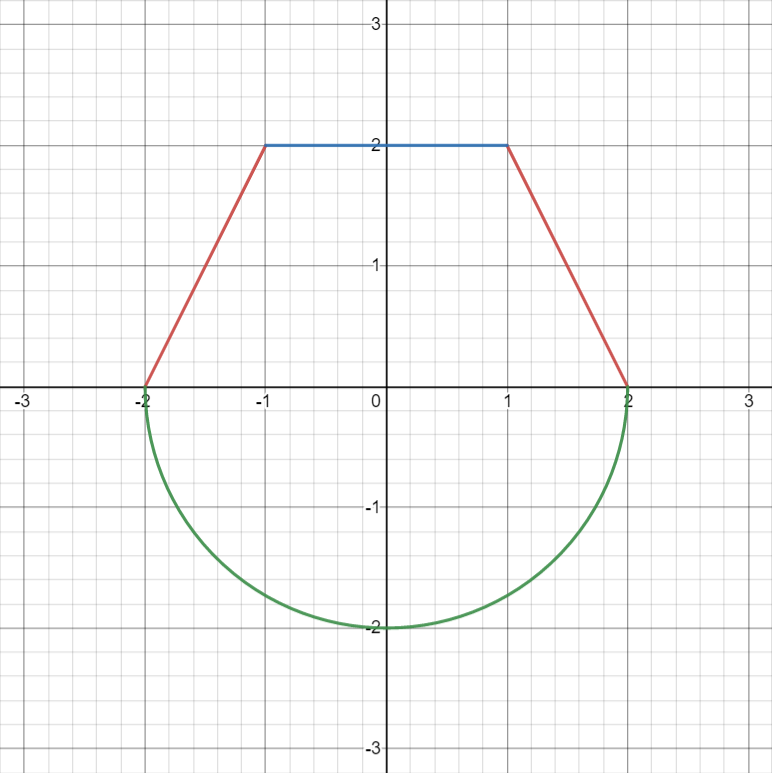
\includegraphics[width=0.8\textwidth]{./Image/Im_05_task2.png}
		\caption{Область, в якій розподілено $\vec\xi$}
		\label{im:task2}
	\end{figure}
	
	Рівняння ліній, що обмежують область \textit{D}:
	$$\begin{cases}
		y=2 & -1 \le x \le 1\\
		y=-2x + 4 & 1 \le x \le 2\\
		y = -\sqrt{4 - x^2} & -2 \le x \le 2\\
		y=2x + 4 & -2 \le x \le -1\\
	\end{cases}$$

	\section{Щільності розподілу координат $\xi_1$ та $\xi_2$}
	
	Знайдемо щільність розподілу за формулою:
	$$f_{\vec \xi}(x, y) = 
	\begin{cases}
		\frac{1}{S_D} & (x, y) \in D\\
		0 & (x, y) \notin D\\
	\end{cases}
	$$
	
	$$S_D = \iint\limits_D dxdy = \int_{-2}^{-1}dx\int_{-\sqrt{4-x^2}}^{2x+4}dy + \int_{-1}^{1}dx\int_{-\sqrt{4-x^2}}^{2}dy + \int_{1}^{2}dx\int_{-\sqrt{4-x^2}}^{-2x+4}dy =$$
	$$ = \int_{-2}^{-1}(2x+4 + \sqrt{4-x^2})dx + \int_{-1}^{1}(2 + \sqrt{4-x^2})dx + \int_{1}^{2}(4- 2x+\sqrt{4-x^2})dx =$$
	$$ = \int_{-2}^{-1}(2x+4)dx + \int_{-1}^{1}2dx + \int_{1}^{2}(4- 2x)dx + \int_{-2}^{2}\sqrt{4-x^2}dx=$$
	$$ = \left.\left(x^2 + 4x\right)\right|_{-2}^{-1} + \left.2x\right|_{-1}^{1} + \left.\left(4x - x^2\right)\right|_{1}^{2} - 4\int_{\pi}^{0}\sin^2{\varphi}d\varphi = $$
	$$ = 1 + 4 + 1 + 2\int_{0}^{\pi}(1 -\cos{2\varphi})d\varphi = 6 + \left.(2\varphi - \sin{2\varphi})\right|_{0}^{\pi} = $$
	$$ = 6 + 2\pi
	$$
	
	В подальшому для обчислення інтегралу $\int\sqrt{4-x^2}dx$ користуватимемось загальною формулою, яка наведена у додатку А.
	
	Позначимо $S_D = 6 + 2\pi$.
	
	Отже, щільність розподілу:
	$$f_{\vec \xi}(x, y) = 
	\begin{dcases}
		\frac{1}{6+2\pi} & (x, y) \in D\\
		0 & (x, y) \notin D\\
	\end{dcases}
	$$
	
	Тепер знайдемо маргінальні щільності координат вектора.
		
	$$f_{\xi_1}(x) = \int_{-\infty}^{\infty}f_{\vec\xi}(x, y)dy =
	\begin{dcases}
		0 & x \le -2\\
		\frac{1}{S_D}\int_{-\sqrt{4-x^2}}^{2x+4}dy & -2 < x \le -1\\
		 \frac{1}{S_D}\int_{-\sqrt{4-x^2}}^{2}dy & -1 < x \le 1\\
		 \frac{1}{S_D}\int_{-\sqrt{4-x^2}}^{-2x+4}dy & 1 < x \le 2\\
		 0 & 2 < x
	\end{dcases}
	$$	
	
	$$f_{\xi_1}(x) = \int_{-\infty}^{\infty}f_{\vec\xi}(x, y)dy =
	\begin{dcases}
		0 & x \le -2\\
		\frac{2x+4+\sqrt{4-x^2}}{6+2\pi} & -2 < x \le -1\\
		\frac{2+\sqrt{4-x^2}}{6+2\pi} & -1 < x \le 1\\
		\frac{4-2x+\sqrt{4-x^2}}{6+2\pi} & 1 < x \le 2\\
		0 & 2 < x
	\end{dcases}
	$$	
	
	Перевірка умови нормування: $\int_{-\infty}^{\infty}f_{\xi_1}(x)dx = 1$.
	
	$$ \int_{-\infty}^{\infty}f_{\xi_1}(x)dx = \dfrac{1}{6+2\pi}\left(\int_{-2}^{-1}(2x+4+\sqrt{4-x^2})dx + \int_{-1}^{1}(2+\sqrt{4-x^2})dx \right) +$$
	$$ + \dfrac{1}{6+2\pi}
	\int_{1}^{2}(4-2x+\sqrt{4-x^2})dx = $$
	$$ = \dfrac{1}{6+2\pi}\left(\int_{-2}^{-1}(2x+4)dx + \int_{-1}^{1}2dx + \int_{1}^{2}(4- 2x)dx + \int_{-2}^{2}\sqrt{4-x^2}dx\right)=$$
	$$ = \dfrac{1}{6+2\pi}\left(\left.\left(x^2 + 4x\right)\right|_{-2}^{-1} + \left.2x\right|_{-1}^{1} + \left.\left(4x - x^2\right)\right|_{1}^{2} - 4\int_{\pi}^{0}\sin^2{\varphi}d\varphi\right) = $$
	$$ = \dfrac{1}{6+2\pi}\left(1 + 4 + 1 + 2\int_{0}^{\pi}(1 -\cos{2\varphi})d\varphi = 6 + \left.(2\varphi - \sin{2\varphi})\right|_{0}^{\pi} \right)= $$
	$$ = \dfrac{6 + 2\pi}{6+2\pi} = 1
	$$
	
	\begin{figure}[H]
		\centering
		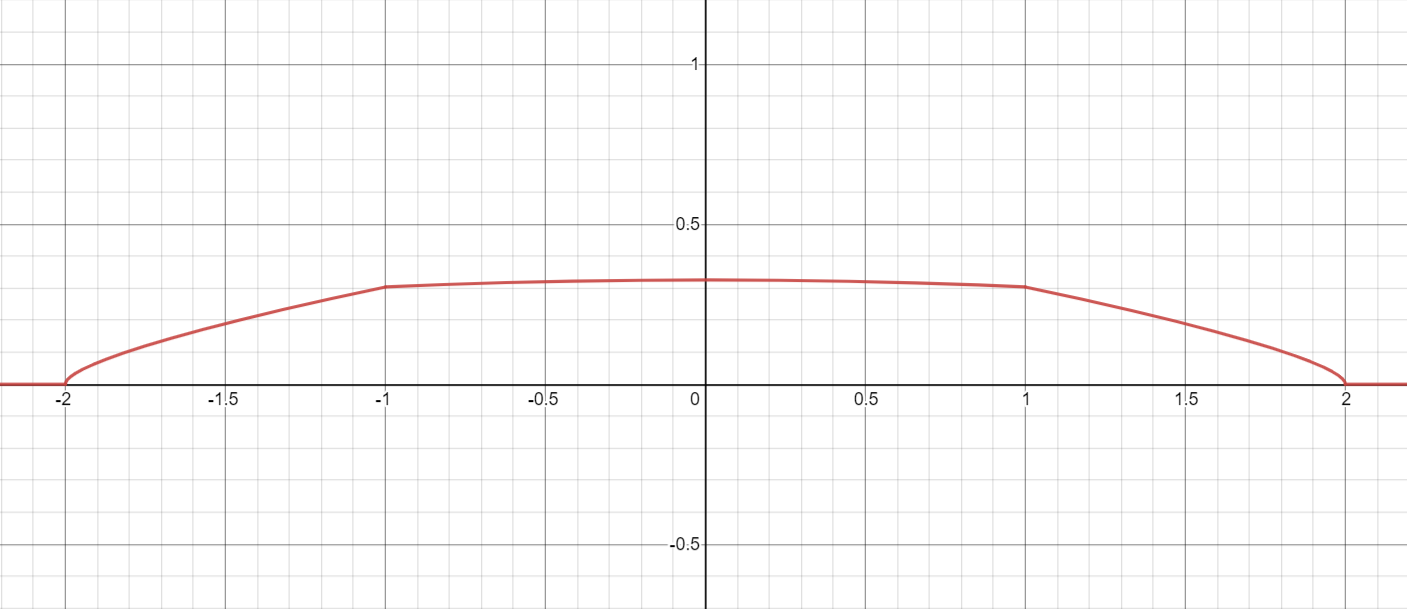
\includegraphics[width=\textwidth]{./Image/Im_06_f1.png}
		\caption{Щільність координати $\xi_1(x)$}
		\label{im:f1}
	\end{figure}
	
	$$f_{\xi_2}(y) = \int_{-\infty}^{\infty}f_{\vec\xi}(x, y)dx =
	\begin{dcases}
		0 & y \le -2\\
		\frac{1}{S_D}\int_{-\sqrt{4-y^2}}^{\sqrt{4-y^2}}dx & -2 < y \le 0\\
		\frac{1}{S_D}\int_{0.5y - 2}^{-0.5y + 2}dx & 0 < y \le 2\\
		0 & 2 < y
	\end{dcases}
	$$
		
	$$f_{\xi_2}(y) = 
	\begin{dcases}
		0 & y \le -2\\
		\dfrac{2\sqrt{4-y^2}}{6+2\pi} & -2 < y \le 0\\
		\frac{4-y}{6+2\pi} & 0 < y \le 2\\
		0 & 2 < y
	\end{dcases}
	$$
	
	Перевірка умови нормування: $\int_{-\infty}^{\infty}f_{\xi_2}(y)dy = 1$.
	
	$$\int_{-\infty}^{\infty}f_{\xi_2}(y)dy = \dfrac{1}{6+2\pi}\left(2\int_{-2}^{0}\sqrt{4-y^2}dy + \int_{0}^{2}(4-y)dy \right) = $$
	$$ = \dfrac{1}{6+2\pi} \left(8\int_{-\frac{\pi}{2}}^{0}\cos^2{\varphi}d\varphi + \left.(4y - \dfrac{y^2}{2})\right|_0^2)\right) =$$ 
	$$ = \dfrac{1}{6+2\pi}\left(4\int_{-\frac{\pi}{2}}^{0}(1+cos{2\varphi})d\varphi + 6\right) = $$
	$$ = \dfrac{1}{6 + 2\pi} \left(\left.\left(4\varphi + 2\sin{2\varphi}\right)\right|_{-\frac{\pi}{2}}^0 + 6\right) = \frac{6 + 2\pi}{6 + 2\pi} = 1 $$
	
	\begin{figure}[H]
		\centering
		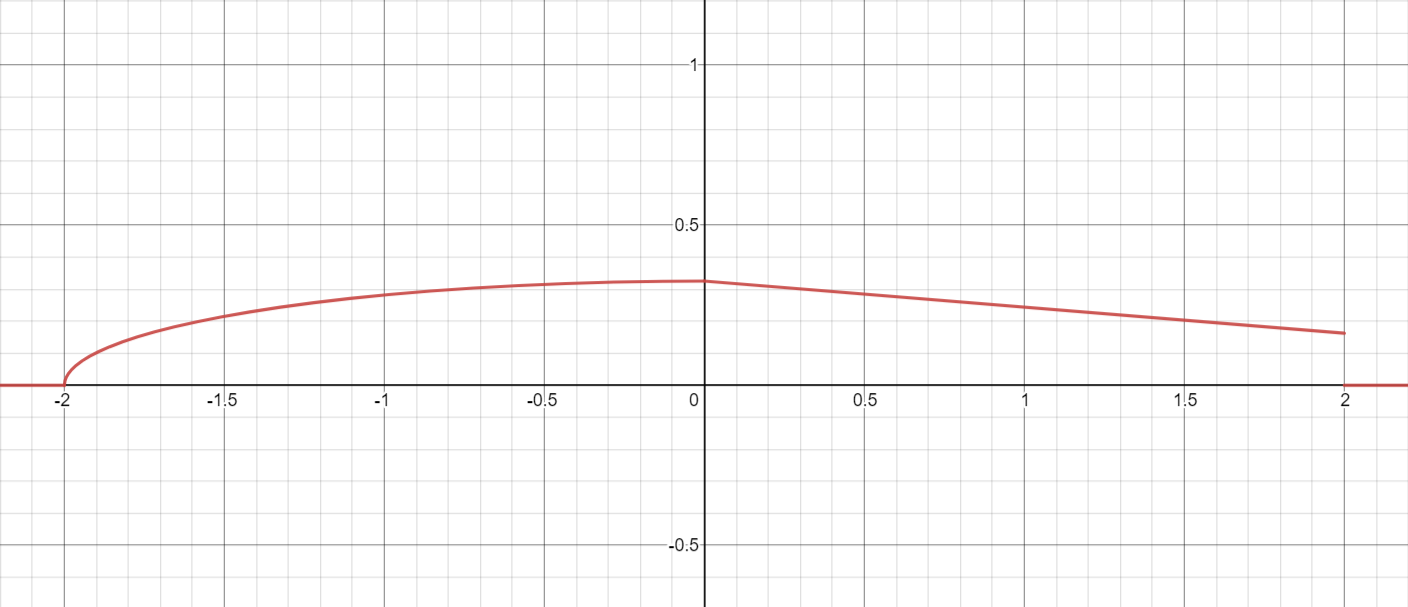
\includegraphics[width=\textwidth]{./Image/Im_07_f2.png}
		\caption{Щільність координати $\xi_2(y)$}
		\label{im:f2}
	\end{figure}
	
	
	\section{Функції розподілу координати $\xi_1$ та $\xi_2$}
	
	Обчислимо функцію розподілу $F_{\xi_1}(x)$ координати $\xi_1$.
	
	$$F_{\xi_1}(x) = \int_{-\infty}^{x}f_{\xi_1}(x)dx$$
	
		$$F_{\xi_1}(x) = \begin{dcases}
		0 & x \le -2\\
		\dfrac{1}{6+2\pi} \int_{-2}^{x}(2s+4+\sqrt{4-s^2})ds& -2 < x \le -1\\
		F_{\xi_1}(-1) + \dfrac{1}{6+2\pi} \int_{-1}^{x}(2+\sqrt{4-s^2})ds & -1 < x \le 1\\
		F_{\xi_1}(1)+\dfrac{1}{6+2\pi} \int_{1}^{x}(4-2s+\sqrt{4-s^2})ds & 1 < x \le 2\\
		1 & 2 < x
	\end{dcases} 
	$$
	
	$$F_{\xi_1}(x) = \begin{dcases}
		0 & x \le -2\\
		\dfrac{x^2 + 4x + 2\arcsin{\frac{x}{2}} + \frac{x}{2}\sqrt{4-x^2} + 4 + \pi}{6+2\pi} & -2 < x \le -1\\
		\dfrac{2x + 2\arcsin{\frac{x}{2}} + \frac{x}{2}\sqrt{4-x^2} + 3 + \pi}{6+2\pi} & -1 < x \le 1\\
		\dfrac{4x - x^2 + 2\arcsin{\frac{x}{2}} + \frac{x}{2}\sqrt{4-x^2}+  2 + \pi}{6+2\pi} & 1 < x \le 2\\
		1 & 2 < x
	\end{dcases} 
	$$
	
	Перевірка неперервності функції розподілу $F_{\xi_1}(x)$ в точках склейки.
	
	$$
	\lim\limits_{-2-0}F_{\xi_1}(x) = 0$$
	$$\lim\limits_{-2+0}F_{\xi_1}(x) = \lim\limits_{-2+0}\left(\dfrac{x^2 + 4x + 2\arcsin{\frac{x}{2}} + \frac{x}{2}\sqrt{4-x^2} + 4 + \pi}{6+2\pi}\right) = $$
	$$ = \dfrac{(-2)^2 + 4(-2) + 2\arcsin{\frac{(-2)}{2}} + \frac{(-2)}{2}\sqrt{4-(-2)^2} + 4 + \pi}{6+2\pi} = $$
	$$ = \dfrac{4 - 8 - \pi + 4 + \pi}{6+2\pi} = 0
	$$
	$$\lim\limits_{-1-0}F_{\xi_1}(x) = \lim\limits_{-1-0} \left(\dfrac{x^2 + 4x + 2\arcsin{\frac{x}{2}} + \frac{x}{2}\sqrt{4-x^2} + 4 + \pi}{6+2\pi}\right) = $$
	$$ =\dfrac{(-1)^2 + 4(-1) + 2\arcsin{\frac{(-1)}{2}} + \frac{(-1)}{2}\sqrt{4-(-1)^2} + 4 + \pi}{6+2\pi} = 
	$$ 
	$$ = \dfrac{1 -4 - \frac{\pi}{3} - \frac{\sqrt{3}}{2} + 4 + \pi}{6+2\pi} = \dfrac{1 + \frac{2\pi}{3} - \frac{\sqrt{3}}{2}}{6+2\pi}
	$$
	$$\lim\limits_{-1+0}F_{\xi_1}(x) = 
	\lim\limits_{-1+0}\left(\dfrac{2x + 2\arcsin{\frac{x}{2}} + \frac{x}{2}\sqrt{4-x^2} + 3 + \pi}{6+2\pi}\right) = 
	$$
	$$= \dfrac{2(-1) + 2\arcsin{\frac{(-1)}{2}} - \frac{1}{2}\sqrt{4-(-1)^2} + 3 + \pi}{6+2\pi} = 
	$$
	$$ \dfrac{-2 -\frac{\pi}{3} - \frac{\sqrt{3}}{2} + 3 + \pi}{6+2\pi} = \dfrac{1  + \frac{2\pi}{3} - \frac{\sqrt{3}}{2}}{6+2\pi}
	$$
	$$ \lim\limits_{1-0}F_{\xi_1}(x) = 
	\lim\limits_{1-0}\left(\dfrac{2x + 2\arcsin{\frac{x}{2}} + \frac{x}{2}\sqrt{4-x^2} + 3 + \pi}{6+2\pi}\right) = 
	$$
	$$ = \dfrac{2 + 2\arcsin{\frac{1}{2}} + \frac{1}{2}\sqrt{4-1^2} + 3 + \pi}{6+2\pi} = 
	$$
	$$ = \dfrac{2 + \frac{\pi}{3} + \frac{\sqrt{3}}{2} + 3 + \pi}{6+2\pi} = \dfrac{5 + \frac{4\pi}{3} + \frac{\sqrt{3}}{2}}{6+2\pi}
	$$
	$$ \lim\limits_{1+0}F_{\xi_1}(x) = 
	\lim\limits_{1+0}\left(\dfrac{4x - x^2 + 2\arcsin{\frac{x}{2}} + \frac{x}{2}\sqrt{4-x^2}+  2 + \pi}{6+2\pi}\right) = 
	$$
	$$ = \dfrac{4 - 1^2 + 2\arcsin{\frac{1}{2}} + \frac{1}{2}\sqrt{4-1^2}+  2 + \pi}{6+2\pi} = 
	$$
	$$ = \dfrac{4 - 1 + \frac{\pi}{3} + \frac{\sqrt{3}}{2}+  2 + \pi}{6+2\pi} = \dfrac{5 + \frac{4\pi}{3} + \frac{\sqrt{3}}{2}}{6+2\pi}
	$$
	$$\lim\limits_{2-0}F_{\xi_1}(x) = 
	\lim\limits_{2-0}\left(\dfrac{4x - x^2 + 2\arcsin{\frac{x}{2}} + \frac{x}{2}\sqrt{4-x^2}+  2 + \pi}{6+2\pi}\right) = 
	$$
	$$ = \dfrac{4(2) - 2^2 + 2\arcsin{\frac{2}{2}} + \frac{2}{2}\sqrt{4-2^2} +  2 + \pi}{6+2\pi} =
	$$
	$$ = \dfrac{8 - 4 + \pi +  2 + \pi}{6+2\pi} = \dfrac{6 + 2\pi}{6+2\pi} = 1
	$$ 
	$$ \lim\limits_{2+0}F_{\xi_1}(x) = 1
	$$
	
	Як видно, в точках склейки значення функції розподілу збігається, отже $F_{\xi_1}(x)$ -- неперервна (це також видно з графіку наведеного на рис.\ref{im:F1}).
	
	\begin{figure}[H]
		\centering
		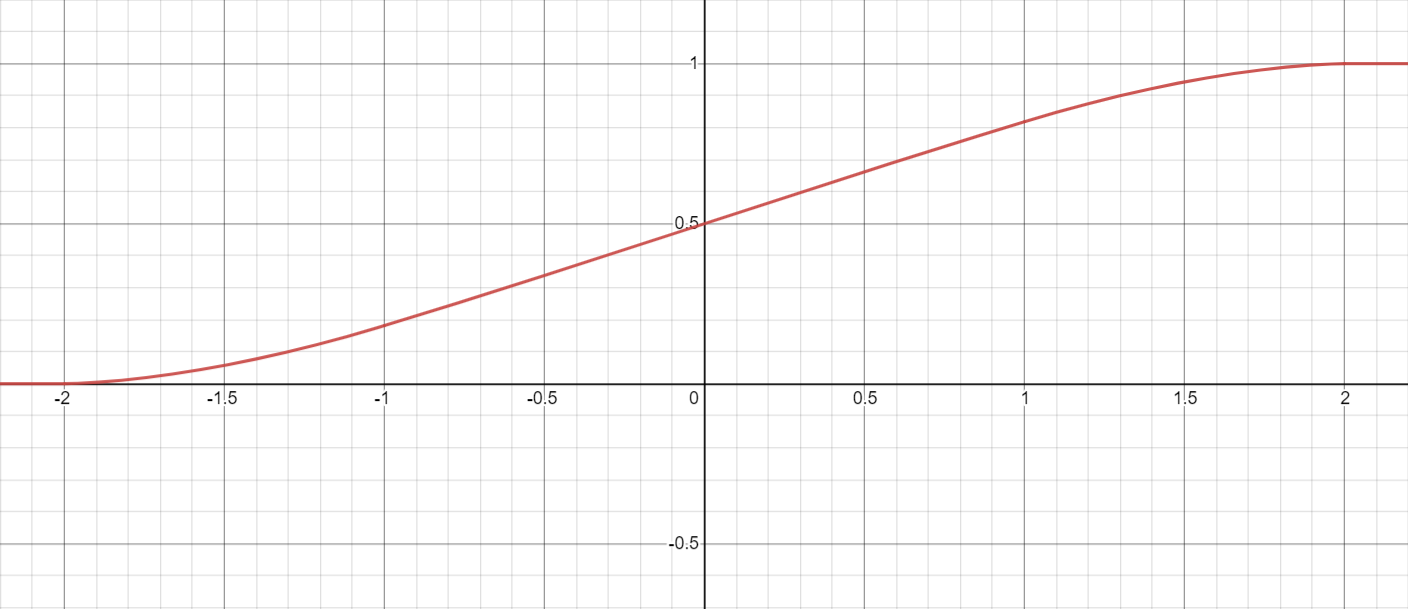
\includegraphics[width=\textwidth]{./Image/Im_08_F1.png}
		\caption{Функція розподілу $F_{\xi_1}(x)$}
		\label{im:F1}
	\end{figure}
	
	Аналогічно обчислимо функцію розподілу $F_{\xi_2}(y)$ координати $\xi_2$.
	
	$$ F_{\xi_2}(y) = 
	\begin{dcases}
			0 & x \le -2\\
			\dfrac{2}{6+2\pi}\int_{-2}^{y}\sqrt{4-y^2}dy & -2 \le y \le 0\\
			\dfrac{1}{6+2\pi}\left(F_{\xi_2}(0) +  \int_{0}^{y}(4-y)dy \right)& 0 \le y \le 2\\
			1 & 2 < y\\
	\end{dcases}
	$$
	
	$$ F_{\xi_2}(y) = 
	\begin{dcases}
		0 & x \le -2\\
		\dfrac{2\arcsin{\frac{x}{2}} + \frac{x}{2}\sqrt{4-x^2} + \pi}{3+\pi} & -2 \le y \le 0\\
		\dfrac{4y - \frac{y^2}{2} + 2\pi}{6+2\pi}& 0 \le y \le 2\\
		1 & 2 < y\\
	\end{dcases}
	$$
	
		Перевірка неперервності функції розподілу $F_{\xi_2}(y)$ в точках склейки.
		
		$$\lim\limits_{-2-0}F_{\xi_2}(y) = 0
		$$
		$$\lim\limits_{-2+0}F_{\xi_2}(y) = \lim\limits_{-2+0}\left(\dfrac{2\arcsin{\frac{x}{2}} + \frac{x}{2}\sqrt{4-x^2} + \pi}{3+\pi}\right) =
		$$
		$$ = \dfrac{2\arcsin{\frac{(-2)}{2}} + \frac{(-2)}{2}\sqrt{4-(-2)^2} + \pi}{3+\pi} = \dfrac{-\pi + \pi}{3+\pi} = 0
		$$
		$$\lim\limits_{0-0}F_{\xi_2}(y) = \lim\limits_{0-0}\left(\dfrac{2\arcsin{\frac{x}{2}} + \frac{x}{2}\sqrt{4-x^2} + \pi}{3+\pi}\right) = 
		$$
		$$ = \dfrac{2\arcsin{\frac{0}{2}} + \frac{0}{2}\sqrt{4-0^2} + \pi}{3+\pi} = \dfrac{0 +0 +\pi}{3+\pi} = \dfrac{\pi}{3+\pi}
		$$
		$$\lim\limits_{0+0}F_{\xi_2}(y) = \lim\limits_{0-0}\left(\dfrac{4y - \frac{y^2}{2} + 2\pi}{6+2\pi}\right) =
		$$
		$$ = \dfrac{4(0) - \frac{0^2}{2} + 2\pi}{6+2\pi} = \dfrac{0 - 0 + 2\pi}{6+2\pi} = \dfrac{2\pi}{6+2\pi} = \dfrac{\pi}{3+\pi}
		$$
		$$ \lim\limits_{2-0}F_{\xi_2}(y) = \lim\limits_{2-0}\left(\dfrac{4(2) - \frac{2^2}{2} + 2\pi}{6+2\pi}\right) =
		$$
		$$ = \dfrac{8 - \frac{4}{2} + 2\pi}{6+2\pi} = \dfrac{8 - 2 + 2\pi}{6+2\pi} = \dfrac{6 + 2\pi}{6+2\pi} = 1
		$$
		$$ \lim\limits_{2+0}F_{\xi_2}(y) = 1
		$$
		
		Як видно, в точках склейки значення функції розподілу збігається, отже $F_{\xi_2}(y)$ -- неперервна (це також видно з графіку наведеного на рис.\ref{im:F2}).
		
		\begin{figure}[H]
			\centering
			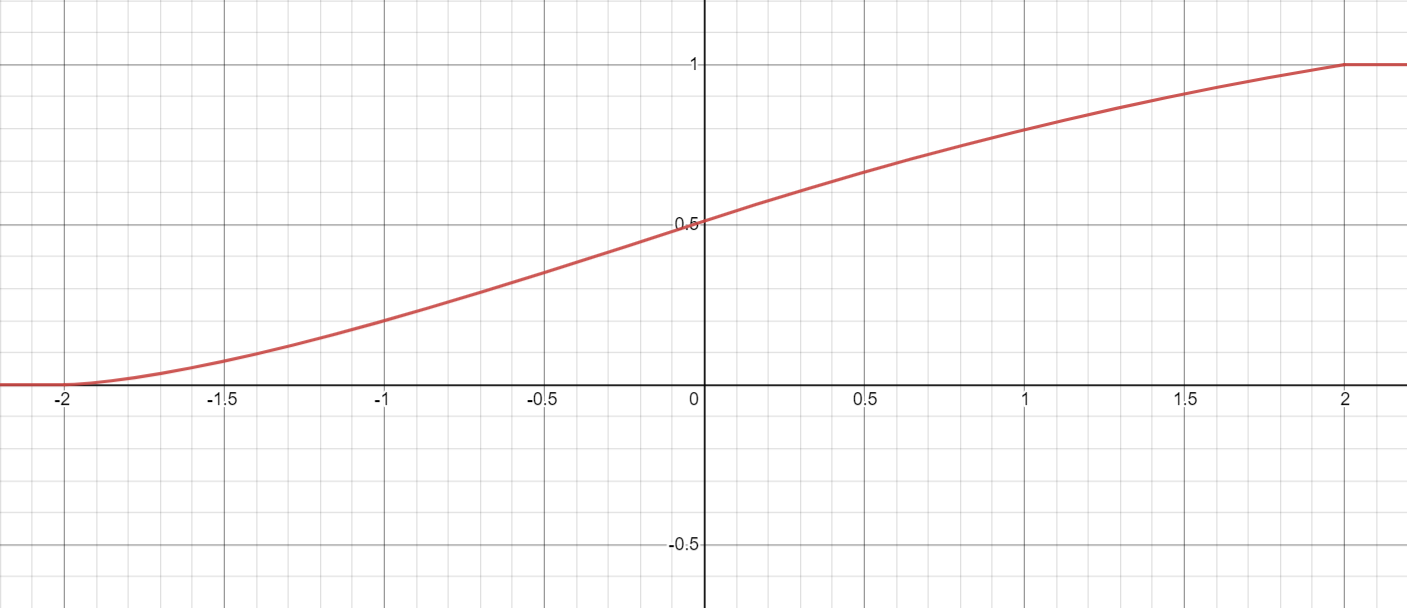
\includegraphics[width=\textwidth]{./Image/Im_09_F2.png}
			\caption{Функція розподілу $F_{\xi_2}(y)$}
			\label{im:F2}
		\end{figure}
	
	
	\section{Сумісна функція розподілу випадкового вектора $\vec\xi$}
	
	
	\section{Математичні сподівання координат. Коваріаційна матриця}
	
	Математичне сподівання $\xi_1$:
	
	$$\mathbb{E}\xi_1 = \int_{-\infty}^{\infty}xf_{\xi_1}(x)dx = \int_{-2}^{-1}\frac{2x^2 + 4x + x\sqrt{4-x^2}}{6+2\pi}dx +
	$$
	$$ + \int_{-1}^{1}\frac{2x + x\sqrt{4-x^2}}{6+2\pi}dx + \int_{1}^{2}\frac{4x-2x^2 + x\sqrt{4-x^2}}{6+2\pi}dx =
	$$
	$$ = \frac{1}{6+2\pi}\left(\left.\left(\frac{2x^3}{3} + 2x^2 \right)\right|_{-2}^{-1} + \left.{x^2}\right|_{-1}^{1} + \left.\left(2x^2 - \frac{2x^3}{3}\right)\right|_{1}^{2} - \right.$$
	$$ - \left.\int_{-2}^{2}\frac{\sqrt{4-x^2}}{2}d(4-x^2)\right) = 
	\frac{1}{6+2\pi} \left(\frac{4}{3} - \frac{8}{3} + 0 + \frac{8}{3} - \frac{4}{3} - \left. \frac{\sqrt{(4-x^2)^3}}{3}\right|_{-2}^2\right) =
	$$
	$$ = \frac{0 - 0}{6 + 2\pi} = 0
	$$
	
	$\mathbb{E}\xi_1 = 0$, як і очікувалось, оскільки область $D$ симетрична відносно осі $OY$.
	
	
	Математичне сподівання $\xi_2$:
	
	$$\mathbb{E}\xi_2 = \int_{-\infty}^{\infty}yf_{\xi_2}(y)dy =\frac{1}{6+2\pi}\left(\int_{-2}^{0}2y\sqrt{4-y^2}dy + \int_{0}^{2}(4y-y^2)dy\right) = 
	$$
	$$ = \frac{1}{6+2\pi}\left(-\int_{-2}^{0}\sqrt{4-y^2}d(4-y^2) + \left.\left(2y^2 - \frac{y^3}{3}\right)\right|_0^2\right) = 
	$$
	$$ = \frac{1}{6+2\pi}\left(\left.\left(-\frac{2\sqrt{(4-y^2)^3}}{3}\right)\right|_{-2}^0 + \frac{16}{3}\right) =
	 \frac{1}{6+2\pi}\left(-\frac{16}{3} + \frac{16}{3}\right) = 0
	$$
	
	Отже, центр розсіювання $\mathbb{E}\vec\xi = (\mathbb{E}\xi_1, \mathbb{E}\xi_2)^T = (0, 0)^T$.
	
	Знайдемо дисперсії.
	
	$$ \mathbb{E}\xi_2^2 = \int_{-\infty}^{\infty}x^2f_{\xi_1}(x)dx = \int_{-2}^{-1}\frac{2x^3 + 4x^2 + x^2\sqrt{4-x^2}}{6+2\pi}dx +
	$$
	$$ + \int_{-1}^{1}\frac{2x^2 + x^2\sqrt{4-x^2}}{6+2\pi}dx + \int_{1}^{2}\frac{4x^2-2x^3 + x^2\sqrt{4-x^2}}{6+2\pi}dx =
	$$
	$$ = \frac{1}{6+2\pi}\left(\left.\left(\frac{x^4}{2} + \frac{4x^3}{3} \right)\right|_{-2}^{-1} + \left.{\frac{2x^3}{3}}\right|_{-1}^{1} + \left.\left(\frac{4x^3}{3} - \frac{x^4}{2}\right)\right|_{1}^{2} - \right.$$
	$$ - \left.\int_{-2}^{2}x^2\sqrt{4-x^2}dx\right) = \left|
	\begin{matrix}
		x = 2\sin{t}\\
		t = \arcsin{\frac{x}{2}}\\
		dx = 2\cos{t}dt\\
		x = -2 \Rightarrow t = -\frac{\pi}{2}\\
		x = 2 \Rightarrow t = \frac{\pi}{2}\\
	\end{matrix}
	\right| = 
	\frac{1}{6+2\pi} \left(-\frac{5}{6} + \frac{8}{3} + \frac{2}{3} + \frac{2}{3} + \right.
	$$ 
	$$ + \frac{8}{3} - \frac{5}{6} + \left.16\int_{-\frac{\pi}{2}}^{\frac{\pi}{2}}\sin^2{t}\cos^2{t}dt \right) = \frac{1}{6+2\pi}\left(5 + 4 \int_{-\frac{\pi}{2}}^{\frac{\pi}{2}}\sin^2{2t}dt\right) =
	$$
	$$ = \frac{1}{6+2\pi}\left(5 + 2\int_{-\frac{\pi}{2}}^{\frac{\pi}{2}}(1 - \cos{4t})dt\right)
	 = \frac{1}{6+2\pi}\left(5 + \left.\left(2t + \frac{\sin{4t}}{2}\right)\right|_{-\frac{\pi}{2}}^{\frac{\pi}{2}}\right) =
	$$
	$$ = \frac{1}{6+2\pi}\left(5 + \pi + \pi + 0 \right) =
	 \frac{5 + 2\pi}{6+2\pi}
	$$
	
	$$\mathbb{D}\xi_1 = \mathbb{E}\xi_1^2 - (\mathbb{E}\xi_1)^2 =\frac{5 + 2\pi}{6+2\pi} 
	$$	
	
	$$\mathbb{E}\xi_2^2 = \int_{-\infty}^{\infty}y^2f_{\xi_2}(y)dy = \frac{1}{6+2\pi}\left(\int_{-2}^{0}2y^2\sqrt{4-y^2}dy + \int_{0}^{2}(4y^2-y^3)dy\right) =$$
	
	При обчисленні $2\int_{-2}^{0}y^2\sqrt{4-y^2}dy$ підставимо одразу кінцеву формулу, яка була знайдена в минулому прикладі.
	
	$$ = \frac{1}{6 + 2\pi}\left(\left.\left(4t + \sin{4t}\right)\right|_{-\frac{\pi}{2}}^{0} + \left.\left(\frac{4y^3}{3} - \frac{y^4}{4}\right)\right|_0^2 \right) = 
	\frac{1}{6 + 2\pi}\left(2\pi + \frac{32}{3} - 4 \right) = 
	$$
	$$ = \frac{2\pi + \frac{20}{3} }{6 + 2\pi}$$
	
	$$\mathbb{D}\xi_2 = \mathbb{E}\xi_2^2 - (\mathbb{E}\xi_2)^2 = \frac{\frac{20}{3} + 2\pi}{6+2\pi}
	$$	
	
	Для побудови коваріаційної матриці знайдемо коваріацію:\\ $cov(\xi_1, \xi_2) = \mathbb{E}\xi_1\xi_2 - \mathbb{E}\xi_1\mathbb{E}\xi_2$
 		
 	$$\mathbb{E}\xi_1\xi_2 = \int_{-\infty}^{\infty}\int_{-\infty}^{\infty}xyf(x, y)dxdy = $$
 	$$ =  \frac{1}{6+2\pi} \left(\int_{-2}^{0}dy\int_{-\sqrt{4-y^2}}^{\sqrt{4-y^2}}yxdx + \int_{0}^{2}dy\int_{0.5y-2}^{2-0.5y}yxdx\right) = 
 	$$
 	$$ = \frac{1}{6+2\pi} \left(\int_{-2}^{0}y\left.\left(\frac{x^2}{2}\right)\right|_{-\sqrt{4-y^2}}^{\sqrt{4-y^2}}dy+ \int_{0}^{2}y\left.\left(\frac{x^2}{2}\right)\right|_{0.5y-2}^{2-0.5y}dy \right)= 
 	$$
 	$$ = \frac{1}{6+2\pi} \left(\int_{-2}^{0}y\left(\frac{4-y^2 - 4 + y^2}{2}\right)dy \right.+ 
 	$$
 	$$ + \left.\int_{0}^{2}y\left(\frac{4 - 2y + 0.25y - 0.25y + 2y - 4}{2}\right)dy\right) = 
 	$$
 	$$ =\frac{1}{6+2\pi}\left(\int_{-2}^{2}y(0)dy\right) = 0$$
 	
 	$$cov(\xi_1, \xi_2) = \mathbb{E}\xi_1\xi_2 - \mathbb{E}\xi_1\mathbb{E}\xi_2 = 0 - 0 = 0$$
 		
 	$cov(\xi_1, \xi_2) = 0$, як і має бути, оскільки область $D$ симетрична відносно осі $OY$. Звідси можна зробити висновок, що величини $\xi_1$ та $\xi_2$ некорельовані, відповідно $r(\xi_1, \xi_2) = 0$. Тоді коваріаційна матриця буде:
 	
 	$$C_{\vec\xi} = \left(  
 	\begin{matrix}
 		\dfrac{5+2\pi}{6+2\pi} & 0\\
 		0 & \dfrac{\frac{20}{3} + 2\pi}{6 + 2\pi}\\
 	\end{matrix}\right)
 	$$
 	
 	Зробимо перевірку невід'ємної визначеності матриці: 
 	
 	$$\det{C_{\vec\xi}}  = \frac{5 + 2\pi}{6+2\pi} \cdot \frac{\frac{20}{3} + 2\pi}{6+2\pi} = \frac{\frac{100}{3} + \frac{70\pi}{3} + 4\pi^2}{36 + 24\pi + 2\pi^2} > 0$$
 	 	
 	\section{Умовні щільності розподілу для кожної координати}
 	
 	
 	
	\chapter*{Додаток А}
	\centering Обчислення інтеграла $\int\sqrt{4-x^2}dx$
	
	$$ \int\sqrt{4-x^2}dx = 2\int\sqrt{1-\dfrac{x^2}{4}}dx  = \left|
	\begin{matrix}
		\dfrac{x}{2} = \sin{t}\\
		t = \arcsin\dfrac{x}{2}\\
		dx = 2\cos{t}dt\\
	\end{matrix}
	\right| = 4\int\sqrt{1-{\sin^2{t}}}\cos{t}dt = 
	$$
	$$ = 4\int\cos^2{t}dt = 2\int(1+\cos{2t})dt = 2t + sin2t + C =
	$$
	$$
	= 2t + 2\sin{t}\cos{t} + C = 2t + 2\sin{t}\sqrt{1-\sin^2{t}} + C = 
	$$
	$$
	= 2\arcsin{\dfrac{x}{2}} + \dfrac{x}{2}\sqrt{4-x^2} + C
	$$
		
\end{document}